\chapter{Preprocessing dei Dati}\label{ch:preprocessing}
% Riferimento principale: Aggarwal, "Data Mining: The Textbook", Cap. 2 (citato nelle slide del corso)

\section{Perché il preprocessing è essenziale}\label{sec:intro-preproc}
Prima di applicare qualsiasi algoritmo di data mining, i dati grezzi devono essere resi \emph{analizzabili}. In pratica, il preprocessing riduce la distanza tra ``dati come sono'' e ``dati come l'algoritmo li richiede''. In assenza di un'adeguata preparazione, anche il miglior algoritmo può fallire o produrre risultati fuorvianti (es.\ feature mal estratte, scale non confrontabili, rumore e outlier che dominano l'analisi).

\paragraph{Quattro obiettivi chiave.}
\begin{enumerate}
  \item \textbf{Estrazione di feature}: ricavare attributi informativi a partire da dati grezzi (log, segnali, immagini, testo, traffico di rete, \ldots), ed eventualmente integrare sorgenti eterogenee in un unico dataset.
  \item \textbf{Portabilità/trasformazione del tipo di dato}: mappare tipi di dato verso rappresentazioni adatte agli algoritmi (es. numerico $\leftrightarrow$ categoriale, testo $\to$ vettori).
  \item \textbf{Data cleaning}: trattare valori mancanti, errori, inconsistenze e outlier; riportare gli attributi su scale confrontabili (scaling/normalizzazione).
  \item \textbf{Riduzione dei dati}: diminuire dimensionalità o volume preservando l'informazione utile (selezione/trasformazione di feature, sampling, PCA/SVD/LSA).
\end{enumerate}

\section{Estrazione di feature}\label{sec:feature}
L'estrazione di feature costruisce un set di attributi più adatti al problema. È fortemente dipendente dal dominio e incide in modo determinante sulla qualità dell'analisi.

\paragraph{Esempi tipici.}
\begin{itemize}
  \item \textbf{Dati sensoriali}: dopo il cleaning, si possono utilizzare direttamente i campioni o trasformarli (es. trasformata di Fourier) per ottenere feature spettrali.
  \item \textbf{Immagini}: matrici di pixel, istogrammi di colore, \emph{edge features}.
  \item \textbf{Web logs}: record testuali formattati da cui si estraggono feature di sessione, frequenze, pattern di navigazione.
  \item \textbf{Traffico di rete}: conteggi, tassi, durate; utili per intrusion detection.
  \item \textbf{Documenti}: rappresentazione \emph{bag-of-words} o pesi TF--IDF (\S\ref{subsec:text2num}).
\end{itemize}

\section{Portabilità dei dati}\label{sec:portabilita}
Gli algoritmi spesso richiedono tipologie di input specifiche; la \emph{portabilità} converte i dati nella forma necessaria. Talvolta la conversione è \emph{lossy} (perdita di informazione): è buona norma esplicitarne il compromesso.

\subsection{Da numerico a categoriale: discretizzazione}\label{subsec:discret}
La discretizzazione suddivide il dominio numerico in intervalli, assegnando a ciascun valore l'etichetta dell'intervallo corrispondente.
\begin{description}
  \item[Equi-width] Intervalli di uguale ampiezza: $[a, a+w), [a+w, a+2w), \ldots$.
  \item[Equi-depth] Intervalli con uguale numerosità attesa (\emph{quantile binning}).
  \item[Equi-log] Intervalli di uguale differenza su scala logaritmica.
\end{description}
\paragraph{Esempio.} Età $\in[0,80]$ in 4 \emph{intervalli} equi-distanti da 20 anni: $[0,20),[20,40),[40,60),[60,80]$. L'età 23 $\mapsto$ intervallo 2.

\subsection{Da categoriale a numerico}\label{subsec:cat2num}
\emph{Label encoding} assegna un intero a categoria, ma introduce un ordine fittizio. Per modelli sensibili all'ordinalità (NN, distanze), si preferisce l'\emph{one-hot encoding}.
\paragraph{Definizione (one-hot).} Per $g$ categorie si rappresenta la categoria $c_i$ con $\mathbf{e}_i\in\{0,1\}^g$, dove $(\mathbf{e}_i)_i=1$ e altrove 0.
\paragraph{Esempio.} Colore $\in\{\texttt{rosso},\texttt{verde},\texttt{blu}\}$: rosso $\to(1,0,0)$; blu $\to(0,0,1)$.

\subsection{Da testo a numerico}\label{subsec:text2num}
Una collezione di $n$ documenti e $d$ termini può essere rappresentata da una matrice \emph{termine-documento} $X\in\mathbb{R}^{d\times n}$, con $x_{tj}$ frequenze (o pesi TF--IDF) del termine $t$ nel documento $j$. La matrice è tipicamente sparsa; tecniche di riduzione (\S\ref{sec:riduzione}) sono utili.

\section{Data cleaning}\label{sec:cleaning}
Il cleaning gestisce mancanze, errori e inconsistenze, e riporta le feature su scale comparabili.

\subsection{Valori mancanti}\label{subsec:missing}
\begin{itemize}
  \item \textbf{Eliminazione di record} con mancanti: semplice, ma rischiosa se i mancanti sono frequenti o non \emph{MCAR} (\emph{Missing Completely At Random}).
  \item \textbf{Imputazione}: media/mediana per attributi numerici; categoria/moda per categoriali; metodi più accurati includono $k$-NN, regressione, EM, modelli generativi. \emph{Nota}: imputazioni errate possono introdurre bias.
  \item \textbf{Gestione nativa}: alcuni algoritmi tollerano i mancanti (es. alberi decisionali con surrogate splits).
\end{itemize}
\paragraph{Mini-esempio (serie temporale).} Per dati temporali/spaziali è comune l'interpolazione (lineare, spline) per colmare piccole lacune.

\subsection{Valori errati e inconsistenze}\label{subsec:errors}
\begin{itemize}
  \item \textbf{Deduplicate/record linkage}: rilevazione e fusione di duplicati (spesso in integrazione di sorgenti).
  \item \textbf{Vincoli di dominio}: coerenza semantica (es. Nazione=\texttt{USA} \(\Rightarrow\) Città \(\neq\) \texttt{Roma}).
  \item \textbf{Outlier}: punti anomali da investigare; non sempre errori, ma potenziali driver del fenomeno.
\end{itemize}

\subsection{Rilevazione di outlier con quantili}\label{subsec:quantili}
Sia $S$ un insieme di valori. Il quantile d'ordine $x\in[0,1]$ è $q_x$ tale che $x\%$ di $S$ è minore di $q_x$ e $(1-x)\%$ maggiore o uguale.
\paragraph{Interquantile range (IQR).} $\mathrm{IQR}=Q_3-Q_1$. La regola classica assegna come outlier i valori
\[
  x< Q_1-1.5\,\mathrm{IQR}\quad \text{oppure}\quad x> Q_3+1.5\,\mathrm{IQR}.
\]
\paragraph{Mini-esempio.} Con $Q_1=10$, $Q_3=22$, $\mathrm{IQR}=12$: soglia bassa $=10-18=-8$, soglia alta $=22+18=40$. Valori $>40$ o $<-8$ sono outlier.

\subsection{Scaling e normalizzazione}\label{subsec:scaling}
Scale diverse rendono gli attributi \emph{non confrontabili} (es. Età vs Salario). La distanza euclidea è dominata dalla scala maggiore. Due standard interventi:
\paragraph{Standardizzazione (z-score).} Per un attributo $A_j$ con media $\mu_j$ e deviazione standard $\sigma_j>0$, ogni valore $x_{pj}$ è trasformato in
\[
  z_{pj}=\frac{x_{pj}-\mu_j}{\sigma_j},\quad \mu_j=\frac{1}{n}\sum_{p=1}^n x_{pj},\quad \sigma_j^2=\frac{1}{n}\sum_{p=1}^n(x_{pj}-\mu_j)^2.
\]
\paragraph{Min--max scaling.} Con $\min_j,\max_j$ valori minimo/massimo osservati di $A_j$,
\[
  y_{pj}=\frac{x_{pj}-\min_j}{\max_j-\min_j}\in[0,1].
\]
\emph{Nota}: il min--max è sensibile agli outlier; lo z-score è più robusto ma non limita l'intervallo.

\section{Riduzione dei dati}\label{sec:riduzione}
Ridurre volume e/o dimensionalità accelera l'analisi e migliora la generalizzazione, a parità d'informazione.

\subsection{Sampling}\label{subsec:sampling}
Costruire un sottoinsieme rappresentativo dei dati.
\begin{itemize}
  \item \textbf{Biased (guidato)}: privilegia porzioni ritenute più informative (es. record recenti in serie temporali).
  \item \textbf{Stratificato}: partiziona il dataset in strati omogenei e campiona proporzionalmente in ogni strato.
\end{itemize}

\subsection{Selezione di feature}\label{subsec:feature-selection}
Rimuovere attributi irrilevanti, ridondanti o rumorosi.
\begin{itemize}
  \item \textbf{Unsupervised}: criteri di ridondanza/varianza, filtri (es. varianza bassa) e metodi embedded.
  \item \textbf{Supervised}: per classificazione, scegliere feature predittive della classe (filtri basati su correlazione/\emph{mutual information}, wrapper, embedded tipo LASSO).
\end{itemize}

\subsection{Riduzione tramite rotazione di assi: PCA}\label{subsec:pca}
La \emph{Principal Component Analysis} cerca una base ortogonale in cui poche dimensioni catturano la maggior parte della varianza.
\paragraph{Matrice di covarianza.} Dato un dataset $D\in\mathbb{R}^{M\times N}$ (righe=record, colonne=attributi), centrato per colonna, la covarianza è $C=\tfrac{1}{M}D^\top D\in\mathbb{R}^{N\times N}$.
\paragraph{Autodecomposizione.} $C=P\,\Lambda\,P^\top$, con colonne di $P$ autovettori ortonormali (componenti principali) e $\Lambda=\mathrm{diag}(\lambda_1\ge\cdots\ge\lambda_N)$ varianze spiegate.
\paragraph{Trasformazione.} Scegliendo $P$ componenti $P_p=[\mathbf{p}_1\,\cdots\,\mathbf{p}_P]$, i dati proiettati sono
\[
  D' = D\,P_p.\label{eq:pca-transform}
\]
\paragraph{Scelta del numero di componenti.} Si usa la frazione di varianza spiegata $\sum_{i=1}^P\lambda_i/\sum_{i=1}^N\lambda_i$ (\emph{es.} soglia 90\%), oppure un grafico a gomito (\emph{scree plot}).
\paragraph{Mini-esempio (intuitivo).} Con due attributi fortemente correlati (es. altezza e apertura delle braccia), la prima componente è circa la bisettrice che massimizza la varianza proiettata; la seconda è ortogonale e a bassa varianza.

\subsection{Singular Value Decomposition (SVD)}\label{subsec:svd}
La SVD decompone una matrice $M\in\mathbb{R}^{n\times d}$ come
\[
  M = U\,\Sigma\,V^\top,
\]
con $U\in\mathbb{R}^{n\times n}$ e $V\in\mathbb{R}^{d\times d}$ ortogonali, e $\Sigma\in\mathbb{R}^{n\times d}$ diagonale non negativa. I valori singolari non nulli sono radici degli autovalori di $M^\top M$; il loro numero è il rango di $M$.
\paragraph{Interpretazione geometrica.} In $\mathbb{R}^2$, un cerchio unitario è ruotato (da $V$), scalato lungo i semiassi (da $\Sigma$) e ri-ruotato (da $U$) in un'ellisse.

\paragraph{Relazione con PCA.} Con dati centrati, PCA e SVD coincidono (sulle direzioni delle colonne). PCA massimizza varianza spiegata; SVD massimizza la norma di Frobenius catturata dall'approssimazione rank-$k$.

\paragraph{Versioni alternative.}
\begin{itemize}
  \item \textbf{Thin SVD} (o economy): rimuove le \emph{colonne} di $U$ e le \emph{righe} di $\Sigma$ in eccesso rispetto alla dimensione minima.
        Per $M\in\mathbb{R}^{m\times n}$ con $m\ge n$: $U_n\in\mathbb{R}^{m\times n}$, $\Sigma_n\in\mathbb{R}^{n\times n}$, $V^{\top}\in\mathbb{R}^{n\times n}$.
        Decomposizione \emph{esatta} ($M=U_n\,\Sigma_n\,V^{\top}$), ma con meno memoria.
        \textit{Uso tipico}: quando $m\gg n$ (o viceversa) e vuoi la SVD senza parti sicuramente nulle.

  \item \textbf{Compact SVD}: elimina \emph{tutte e sole} le righe/colonne di $\Sigma$ associate a valori singolari \emph{nulli}
        e, di conseguenza, le colonne di $U$ e le righe di $V^{\top}$ corrispondenti.
        Se $\mathrm{rank}(M)=r<\min(m,n)$: $U_r\in\mathbb{R}^{m\times r}$, $\Sigma_r\in\mathbb{R}^{r\times r}$, $V_r^{\top}\in\mathbb{R}^{r\times n}$.
        Decomposizione ancora \emph{esatta}.
        \textit{Uso tipico}: matrici a rango basso (colonne/righe dipendenti), per togliere zeri inutili.

  \item \textbf{Truncated SVD} (rank-$k$): mantiene solo i \emph{primi} $k$ valori singolari ($k<r$) e tronca il resto:
        $U_k\in\mathbb{R}^{m\times k}$, $\Sigma_k\in\mathbb{R}^{k\times k}$, $V_k^{\top}\in\mathbb{R}^{k\times n}$.
        Decomposizione \emph{non esatta}: $M\approx U_k\,\Sigma_k\,V_k^{\top}$, migliore approssimazione a rango $k$ (in norma 2/Frobenius).
        \textit{Uso tipico}: riduzione dimensionale, denoising, LSA/LSI, raccomandazione (si conserva la maggior parte della “energia”).
\end{itemize}


\begin{figure}[htbp]
  \centering
  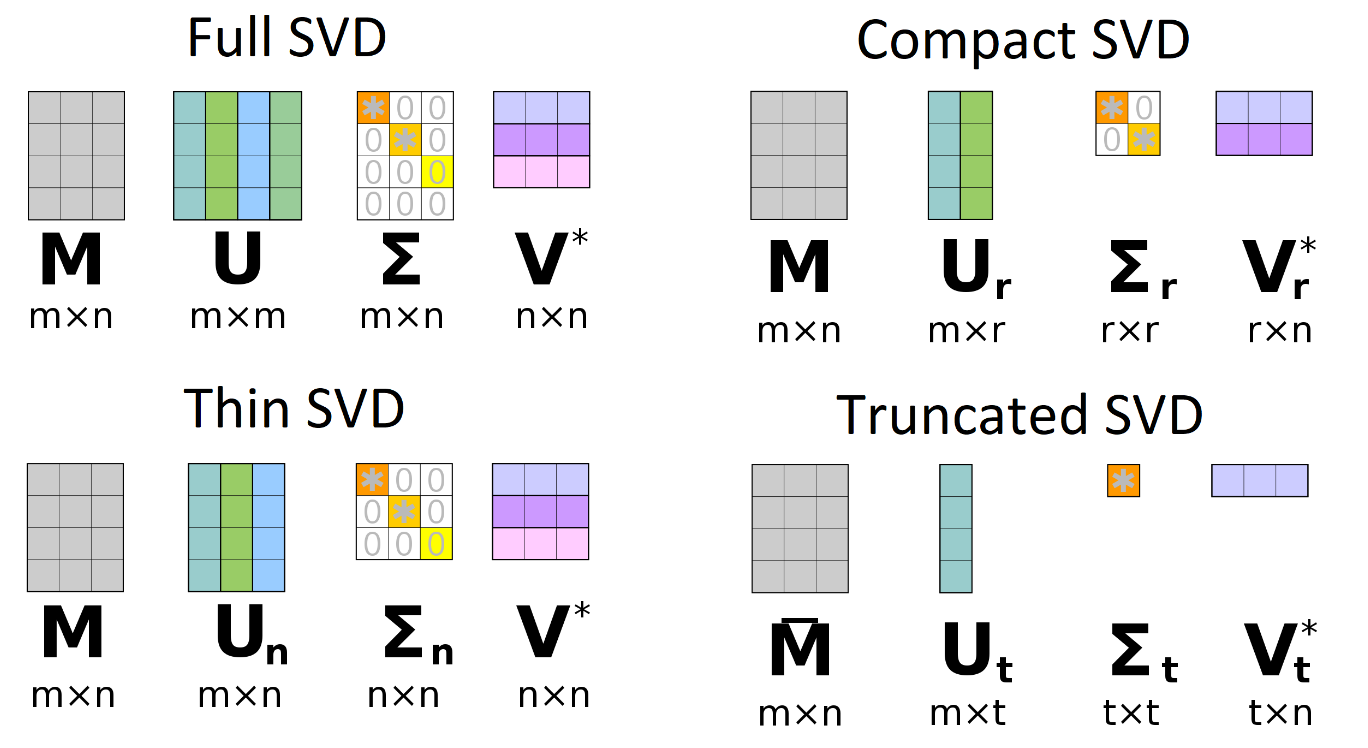
\includegraphics[width=\textwidth]{images/SVD.png}
  \caption{Confronto tra varianti della SVD.
  Full: $U\in\mathbb{R}^{m\times m}$, $\Sigma\in\mathbb{R}^{m\times n}$, $V^{\top}\in\mathbb{R}^{n\times n}$.
  Compact/Thin: $U_r\in\mathbb{R}^{m\times r}$, $\Sigma_r\in\mathbb{R}^{r\times r}$, $V_r^{\top}\in\mathbb{R}^{r\times n}$.
  Truncated: $U_t\in\mathbb{R}^{m\times t}$, $\Sigma_t\in\mathbb{R}^{t\times t}$, $V_t^{\top}\in\mathbb{R}^{t\times n}$ con $t<r$.}
  \label{fig:svd-variants}
\end{figure}

\subsection{Latent Semantic Analysis (LSA)}\label{subsec:lsa}
LSA applica la SVD alla matrice termine-documento (\S\ref{subsec:text2num}). Troncando ai primi $k$ valori singolari si ottiene uno spazio semantico di bassa dimensione che attenua sinonimia/rumore e migliora il recupero di informazione.

\section{Riduzione per trasformazione dei dati}\label{sec:riduzione-trasf}
Ridurre dimensionalità trasformando i dati in forme più compatte e \emph{strutturate}:
\begin{itemize}
  \item \textbf{Serie temporali}: trasformata di Fourier, trasformata wavelet di Haar.
  \item \textbf{Grafi}: embedding spettrali/\emph{multidimensional scaling} per preservare distanze/similarità tra nodi.
\end{itemize}